\subsection{Ablation Studies}
\label{abl:loss}

To assess the individual contributions of the loss functions and spectral bands to the model's reconstruction capability, we conducted two ablation studies. All models were trained using identical hyperparameters and datasets (20\% of the winter subset) to ensure fair comparison.

\subsubsection{Impact of Loss Components}
\label{subsec:ablation_loss}

We evaluated four training configurations to isolate the effects of structural ($\mathcal{L}_{\text{SSIM}}$) and perceptual ($\mathcal{L}_{\text{LPIPS}}$) losses against a baseline adversarial setup:
\begin{enumerate}
    \item $\mathcal{L}_{\text{GAN}} + \mathcal{L}_{\text{L1}}$,
    \item $\mathcal{L}_{\text{GAN}} + \mathcal{L}_{\text{L1}} + \mathcal{L}_{\text{SSIM}}$,
    \item $\mathcal{L}_{\text{GAN}} + \mathcal{L}_{\text{L1}} + \mathcal{L}_{\text{LPIPS}}$, and
    \item the full objective: $\mathcal{L}_{\text{GAN}} + \mathcal{L}_{\text{L1}} + \mathcal{L}_{\text{SSIM}} + \mathcal{L}_{\text{LPIPS}}$.
\end{enumerate}

Table~\ref{tab:ablation_quantitative} summarizes the quantitative results. The baseline configuration ($\mathcal{L}_{\text{GAN}} + \mathcal{L}_{\text{L1}}$) yields the lowest performance across most metrics. This deficiency is also visually apparent, as the generated images lack textural detail (see Fig.~\ref{fig:ablation_samples}b).

Integrating $\mathcal{L}_{\text{SSIM}}$ yields the highest quantitative scores for SSIM and PSNR. However, qualitative inspection reveals that this configuration suffers from perceptual inconsistencies and reduced realism (Fig.~\ref{fig:ablation_samples}c). This aligns with prior findings that SSIM may overemphasize low-level intensity matching at the expense of high-frequency texture fidelity~\cite{nvidia_Understanding_SSIM}. Conversely, incorporating $\mathcal{L}_{\text{LPIPS}}$ significantly improves edge retention and textural realism (Fig.~\ref{fig:ablation_samples}d), reflected in the best LPIPS score of 0.213, though at the cost of slight color deviations compared to the SSIM-based model.

The full combination of losses achieves the optimal trade-off. It maintains competitive pixel-level accuracy (MAE/RMSE) while ensuring structural coherence and perceptual realism, as evidenced in Fig.~\ref{fig:ablation_samples}(e). However, it introduces slight smoothing compared to the LPIPS-only configuration, a tendency likely driven by $\mathcal{L}_{\text{SSIM}}$. This confirms the necessity of a composite loss function that balances the sharpening effect of LPIPS with the structural regularization of SSIM for effective SAR-to-optical translation, consistent with Similar results reported in~\cite{s2o_ViT_cGAN, CR_RS_GAN_s2o}.

\begin{table}[!htbp]
    \centering
    \caption{Quantitative ablation results across loss configurations. Best values are in \textbf{bold}.}
    \label{tab:ablation_quantitative}
    % \resizebox{\columnwidth}{!}{%
        \begin{tabular}{lcccccc}
            \toprule
            \textbf{Configuration} & \textbf{SSIM $\uparrow$} & \textbf{PSNR $\uparrow$} & \textbf{LPIPS $\downarrow$} & \textbf{SAM~(°) $\downarrow$} & \textbf{MAE $\downarrow$} & \textbf{RMSE $\downarrow$} \\
            \midrule
            $\mathcal{L}_{\text{GAN}} + \mathcal{L}_{\text{L1}}$ & 0.820 & 26.38 & 0.287 & 7.88 & 229 & 441 \\
            + $\mathcal{L}_{\text{SSIM}}$ & \textbf{0.862} & \textbf{27.67} & 0.399 & \textbf{6.67} & 198 & \textbf{380} \\
            + $\mathcal{L}_{\text{LPIPS}}$ & 0.842 & 27.58 & \textbf{0.213} & 7.05 & 201 & 385 \\
            Full Combination & 0.859 & 27.65 & 0.224 & 6.71 & \textbf{195} & 382 \\
            \bottomrule
        \end{tabular}%
    % }
\end{table}

\begin{figure}[!htbp]
    \centering
    \setlength{\tabcolsep}{1pt}
    \renewcommand{\arraystretch}{0.5}
    % Grid: 6 columns, responsive width
    \begin{tabular}{cccccc}
        \scriptsize (a) SAR & \scriptsize (b) Base & \scriptsize (c) +SSIM & \scriptsize (d) +LPIPS & \scriptsize (e) Full & \scriptsize (f) GT \\
        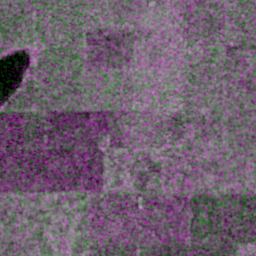
\includegraphics[width=0.16\columnwidth]{../latex_source_code/img/ablation/sample_1/sar.png} &
        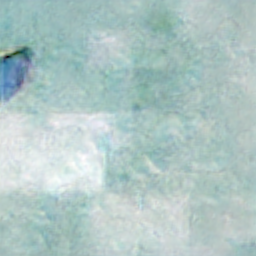
\includegraphics[width=0.16\columnwidth]{../latex_source_code/img/ablation/sample_1/none.png} &
        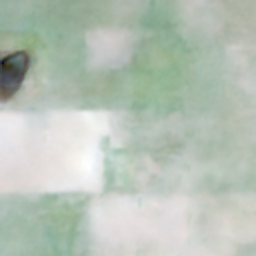
\includegraphics[width=0.16\columnwidth]{../latex_source_code/img/ablation/sample_1/ssim.png} &
        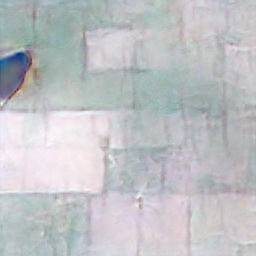
\includegraphics[width=0.16\columnwidth]{../latex_source_code/img/ablation/sample_1/lpips.png} &
        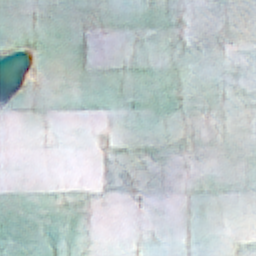
\includegraphics[width=0.16\columnwidth]{../latex_source_code/img/ablation/sample_1/all.png} &
        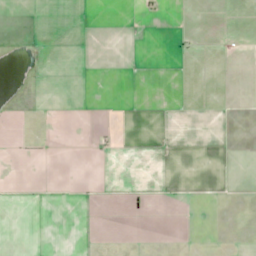
\includegraphics[width=0.16\columnwidth]{../latex_source_code/img/ablation/sample_1/gt.png} \\
        
        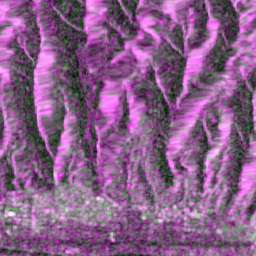
\includegraphics[width=0.16\columnwidth]{../latex_source_code/img/ablation/sample_2/sar.png} &
        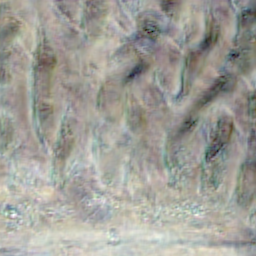
\includegraphics[width=0.16\columnwidth]{../latex_source_code/img/ablation/sample_2/none.png} &
        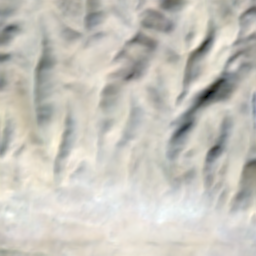
\includegraphics[width=0.16\columnwidth]{../latex_source_code/img/ablation/sample_2/ssim.png} &
        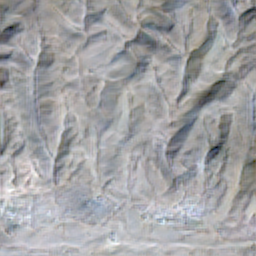
\includegraphics[width=0.16\columnwidth]{../latex_source_code/img/ablation/sample_2/lpips.png} &
        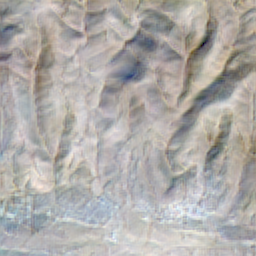
\includegraphics[width=0.16\columnwidth]{../latex_source_code/img/ablation/sample_2/all.png} &
        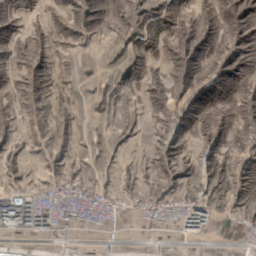
\includegraphics[width=0.16\columnwidth]{../latex_source_code/img/ablation/sample_2/gt.png} \\
        
        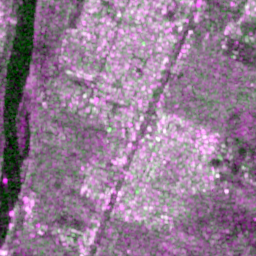
\includegraphics[width=0.16\columnwidth]{../latex_source_code/img/ablation/sample_3/sar.png} &
        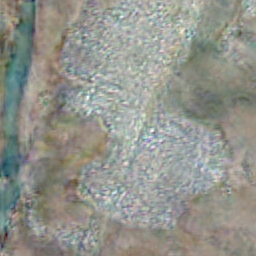
\includegraphics[width=0.16\columnwidth]{../latex_source_code/img/ablation/sample_3/none.png} &
        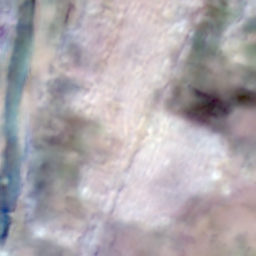
\includegraphics[width=0.16\columnwidth]{../latex_source_code/img/ablation/sample_3/ssim.png} &
        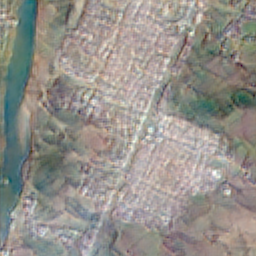
\includegraphics[width=0.16\columnwidth]{../latex_source_code/img/ablation/sample_3/lpips.png} &
        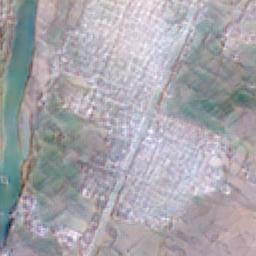
\includegraphics[width=0.16\columnwidth]{../latex_source_code/img/ablation/sample_3/all.png} &
        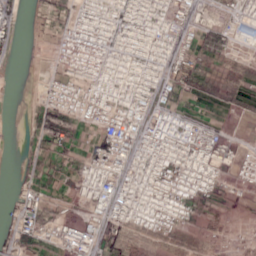
\includegraphics[width=0.16\columnwidth]{../latex_source_code/img/ablation/sample_3/gt.png} \\
    \end{tabular}
    \caption{Visual comparison of loss configurations. (a) Input SAR, (b) Baseline ($\mathcal{L}_{\text{GAN}}{+}\mathcal{L}_{\text{L1}}$), (c) Baseline w/ SSIM, (d) Baseline w/ LPIPS, (e) Proposed full loss, (f) Ground Truth.}
    \label{fig:ablation_samples}
\end{figure}

\subsubsection{Influence of 60m Spectral Bands}
\label{subsec:ablation_60m}
Sentinel-2 includes three 60\,m resolution bands (B1, B9, B10) primarily used for atmospheric correction. We hypothesized that including these lower-resolution bands might introduce noise or training instability due to upsampling artifacts, since they were resampled to 10\,m. To test this, we trained a model strictly excluding these bands.

Contrary to this hypothesis, excluding the 60\,m bands did not improve performance. Instead, radiometric fidelity decreased, with both SSIM and PSNR dropping compared to the full 13-band model (Table~\ref{tab:ablation_excluding_60m}). Interestingly, the Spectral Angle Mapper (SAM) score improved slightly when excluding these bands (6.33° vs. 6.71°). This indicates a trade-off: the model trained on fewer bands learned tighter spectral relationships among the remaining subsets (improving SAM) but lacks the enhanced image quality derived from the atmospheric correction information in the 60\,m bands. It is worth noting, however, that these differences are marginal. Similarly, qualitative inspection in Figure~\ref{fig:ablation_excluding_60m_qualitative} reveals only subtle differences in favour of including the full spectrum.

\begin{table}[!htbp]
    \centering
    \caption{Performance comparison: All 13 bands vs. excluding 60\,m bands (B1, B9, B10).}
    \label{tab:ablation_excluding_60m}
    \begin{tabular}{lccc}
        \toprule
        \textbf{Setting} & \textbf{SSIM $\uparrow$} & \textbf{PSNR (dB) $\uparrow$} & \textbf{SAM~(°) $\downarrow$} \\
        \midrule
        All 13 bands & \textbf{0.859} & \textbf{27.65} & 6.71 \\
        Excluding 60m & 0.826 & 26.47 & \textbf{6.33} \\
        \bottomrule
    \end{tabular}
\end{table}

\begin{figure}[!htbp]
    \centering
    \setlength{\tabcolsep}{2pt}
    \renewcommand{\arraystretch}{0.5}
    \begin{tabular}{cccc}
        \scriptsize (a) SAR & \scriptsize (b) No 60m & \scriptsize (c) Full (13 Bands) & \scriptsize (d) GT \\
        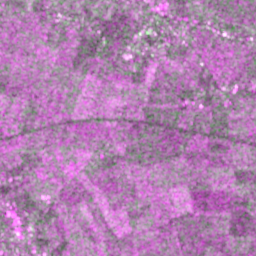
\includegraphics[width=0.23\columnwidth]{../latex_source_code/img/exclusion_60_m/bands10/sample_000034_sar_pseudo.png} &
        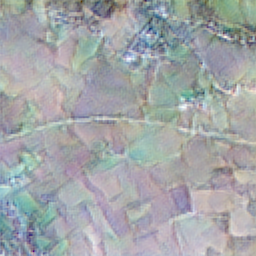
\includegraphics[width=0.23\columnwidth]{../latex_source_code/img/exclusion_60_m/bands10/sample_000034_pred_rgb.png} &
        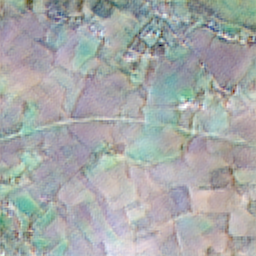
\includegraphics[width=0.23\columnwidth]{../latex_source_code/img/exclusion_60_m/bands13/sample_000034_pred_rgb.png} &
        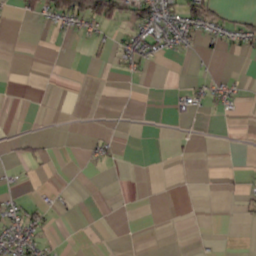
\includegraphics[width=0.23\columnwidth]{../latex_source_code/img/exclusion_60_m/bands10/sample_000034_true_rgb.png} \\
        
        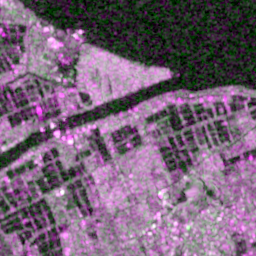
\includegraphics[width=0.23\columnwidth]{../latex_source_code/img/exclusion_60_m/bands10/sample_000050_sar_pseudo.png} &
        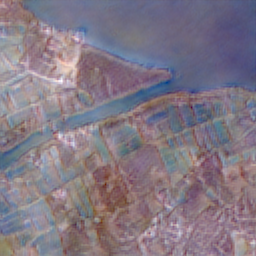
\includegraphics[width=0.23\columnwidth]{../latex_source_code/img/exclusion_60_m/bands10/sample_000050_pred_rgb.png} &
        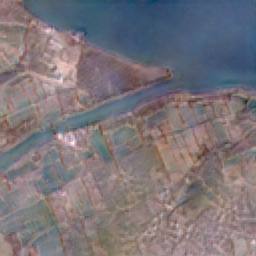
\includegraphics[width=0.23\columnwidth]{../latex_source_code/img/exclusion_60_m/bands13/sample_000050_pred_rgb.png} &
        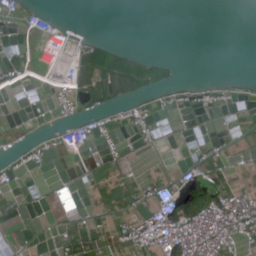
\includegraphics[width=0.23\columnwidth]{../latex_source_code/img/exclusion_60_m/bands10/sample_000050_true_rgb.png} \\
        
         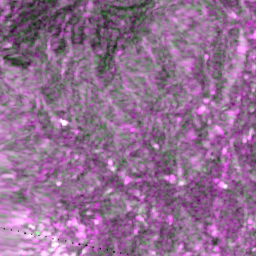
\includegraphics[width=0.23\columnwidth]{../latex_source_code/img/exclusion_60_m/bands10/sample_000010_sar_pseudo.png} &
        
\includegraphics[width=0.23\columnwidth]{../latex_source_code/img/exclusion_60_m/bands10/sample_000010_pred_rgb.png} &
        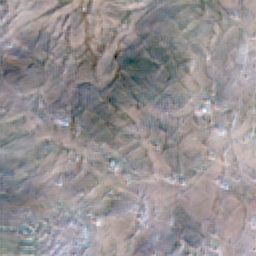
\includegraphics[width=0.23\columnwidth]{../latex_source_code/img/exclusion_60_m/bands13/sample_000010_pred_rgb.png} &
        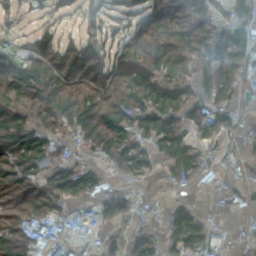
\includegraphics[width=0.23\columnwidth]{../latex_source_code/img/exclusion_60_m/bands10/sample_000010_true_rgb.png} \\
    \end{tabular}
    \caption{Qualitative results comparing models trained with and without the 60\,m bands. (a) SAR input, (b) 10-band model output, (c) 13-band model output, (d) Ground Truth.}
    \label{fig:ablation_excluding_60m_qualitative}
\end{figure}

This trend is further confirmed by the per-band analysis in Table~\ref{tab:ablation_excluding_60m_per_band}. While SSIM remains relatively stable across configurations, PSNR drops for nearly all 10\,m and 20\,m bands when the atmospheric bands are removed, although the absolute differences are small.

\begin{table}[!htbp]
    \centering
    \caption{Per-band performance comparison. \textbf{No 60m}: Model trained without B1, B9, B10. \textbf{13}: Full model.}
    \label{tab:ablation_excluding_60m_per_band}
    \begin{tabular}{lcccc}
    \toprule
    \textbf{Band} & \textbf{SSIM (No 60m)} & \textbf{SSIM (13)} & \textbf{PSNR (No 60m)} & \textbf{PSNR (13)} \\
    \midrule
    B1   & ---    & 0.9634 & ---    & 29.749 \\
    B2 & \textbf{0.9431} & 0.9430 & \textbf{34.15} & 34.06 \\
    B3 & \textbf{0.9064} & 0.9060 & 31.69 & \textbf{31.72} \\
    B4 & \textbf{0.8348} & 0.8340 & 28.04 & \textbf{28.15} \\
    B5 & 0.8707 & \textbf{0.8729} & 28.10 & \textbf{28.26} \\
    B6 & 0.8199 & \textbf{0.8231} & 26.74 & \textbf{26.93} \\
    B7 & 0.7890 & \textbf{0.7925} & 25.69 & \textbf{25.88} \\
    B8 & 0.7375 & \textbf{0.7416} & 25.53 & \textbf{25.74} \\
    B8A & 0.7687 & \textbf{0.7722} & 25.10 & \textbf{25.31} \\
    B9   & ---    & 0.8666 & ---    & 24.617 \\
    B10  & ---    & 0.8826 & ---    & 24.571 \\
    B11 & 0.7774 & \textbf{0.7809} & 23.40 & \textbf{23.73} \\
    B12 & 0.8034 & \textbf{0.8073} & 24.96 & \textbf{25.26} \\
    \bottomrule
    \end{tabular}
\end{table}
